\documentclass[aspectratio=43]{beamer}

% Text packages to stop warnings
\usepackage{lmodern}
\usepackage{textcomp}
\usepackage{ulem}
\usepackage[utf8]{inputenc}
\usepackage[T1]{fontenc}
\usepackage{alltt}

\usepackage{listings}
\usepackage{tikz}
\usetikzlibrary{arrows,decorations.pathreplacing,positioning}

% Themes
\usetheme{Boadilla}
\setbeamertemplate{footline}[page number]{}
\setbeamertemplate{navigation symbols}{}

% Suppress the navigation bar
\beamertemplatenavigationsymbolsempty

\newenvironment{changemargin}[1]{% 
  \begin{list}{}{% 
    \setlength{\topsep}{0pt}% 
    \setlength{\leftmargin}{#1}% 
    \setlength{\rightmargin}{1em}
    \setlength{\listparindent}{\parindent}% 
    \setlength{\itemindent}{\parindent}% 
    \setlength{\parsep}{\parskip}% 
  }% 
  \item[]}{\end{list}} 

\lstset{basicstyle=\scriptsize, frame=single}

\lstdefinelanguage{JavaScript}{
  keywords={typeof, new, true, false, catch, function, return, null, catch, switch, var, if, in, while, do, else, case, break},
  keywordstyle=\color{blue}\bfseries,
  ndkeywords={class, export, boolean, throw, implements, import, this},
  ndkeywordstyle=\color{darkgray}\bfseries,
  identifierstyle=\color{black},
  sensitive=false,
  comment=[l]{//},
  morecomment=[s]{/*}{*/},
  commentstyle=\color{purple}\ttfamily,
  stringstyle=\color{red}\ttfamily,
  morestring=[b]',
  morestring=[b]"
}

\title{Lecture 27---Profiler Lies}
\subtitle{ECE 459: Programming for Performance}
\date{March 13, 2015}

% note: this worked quite well after handing back midterms (10 minutes) and before course evaluations (15 minutes), i.e. a 25 minute lecture
\begin{document}
%%%%%%%%%%%%%%%%%%%%%%%%%%%%%%%%%%%%%%%%%%%%%%%%%%%%%%%%%%%%%%%%%%%%%%%%%%%%%%%%
\begin{frame}[plain]
  \titlepage
\end{frame}
%%%%%%%%%%%%%%%%%%%%%%%%%%%%%%%%%%%%%%%%%%%%%%%%%%%%%%%%%%%%%%%%%%%%%%%%%%%%%%%%

\part{Lies about Calling Context}

%%%%%%%%%%%%%%%%%%%%%%%%%%%%%%%%%%%%%%%%%%%%%%%%%%%%%%%%%%%%%%%%%%%%%%%%%%%%%%%%
\begin{frame}
  \partpage
\end{frame}
%%%%%%%%%%%%%%%%%%%%%%%%%%%%%%%%%%%%%%%%%%%%%%%%%%%%%%%%%%%%%%%%%%%%%%%%%%%%%%%%

%%%%%%%%%%%%%%%%%%%%%%%%%%%%%%%%%%%%%%%%%%%%%%%%%%%%%%%%%%%%%%%%%%%%%%%%%%%%%%%%
\begin{frame}
  \frametitle{gprof and KCacheGrind}
  
  \begin{changemargin}{2cm}
    Who can we trust?\\[1em]

    Some profiler results are real. \\
    Other results are interpolated, and perhaps wrong.
  \end{changemargin}

  \begin{center}
    Reference: Yossi Kreinin,\\
  \tiny
  \url{http://www.yosefk.com/blog/how-profilers-lie-the-cases-of-gprof-and-kcachegrind.html}
  \end{center}

\end{frame}
%%%%%%%%%%%%%%%%%%%%%%%%%%%%%%%%%%%%%%%%%%%%%%%%%%%%%%%%%%%%%%%%%%%%%%%%%%%%%%%%

%%%%%%%%%%%%%%%%%%%%%%%%%%%%%%%%%%%%%%%%%%%%%%%%%%%%%%%%%%%%%%%%%%%%%%%%%%%%%%%%
\begin{frame}[fragile]
  \frametitle{Running Example}

  \begin{center}
  \begin{minipage}{.7\textwidth}
\begin{lstlisting}
void work(int n) {
  volatile int i=0; //don't optimize away
  while(i++ < n);
}
void easy() { work(1000); }
void hard() { work(1000*1000*1000); }
int main() { easy(); hard(); }
\end{lstlisting}
  \end{minipage}
  \end{center}
  
\end{frame}
%%%%%%%%%%%%%%%%%%%%%%%%%%%%%%%%%%%%%%%%%%%%%%%%%%%%%%%%%%%%%%%%%%%%%%%%%%%%%%%%

%%%%%%%%%%%%%%%%%%%%%%%%%%%%%%%%%%%%%%%%%%%%%%%%%%%%%%%%%%%%%%%%%%%%%%%%%%%%%%%%
\begin{frame}[fragile]
  \frametitle{Running the Running Example}

\begin{alltt}
[plam@lynch L27]\$ gprof ./try gmon.out
Flat profile:

Each sample counts as 0.01 seconds.
  \%   cumulative   self              self     total           
 time   seconds   seconds    calls  ms/call  ms/call  name    
101.30      1.68     1.68        2   840.78   840.78  work
  0.00      1.68     0.00        1     0.00   \alert{840.78}  easy
  0.00      1.68     0.00        1     0.00   \alert{840.78}  hard
\end{alltt}

\begin{changemargin}{2cm}
  That's not right! \\
  {\tt easy} takes $\approx$ 0s, {\tt hard} takes 1.68s.
\end{changemargin}
\end{frame}
%%%%%%%%%%%%%%%%%%%%%%%%%%%%%%%%%%%%%%%%%%%%%%%%%%%%%%%%%%%%%%%%%%%%%%%%%%%%%%%%

%%%%%%%%%%%%%%%%%%%%%%%%%%%%%%%%%%%%%%%%%%%%%%%%%%%%%%%%%%%%%%%%%%%%%%%%%%%%%%%%
\begin{frame}[fragile]
  \frametitle{What's Wrong?}

  \begin{changemargin}{2cm}
    Need to understand how {\tt gprof} works.\\[1em]
    \begin{itemize}
    \item
      \begin{tabbing}
      {\bf profil()}: \= asks glibc to record which instruction \\
      \> is currently executing
      (100$\times$/second).
      \end{tabbing}
    \item
      \begin{tabbing}
        {\bf mcount()}: \= records call graph edges;\\
        \> called by {\tt -pg} instrumentation.
      \end{tabbing}
    \end{itemize}
~\\
    {\bf profil} information is statistical; \\
    {\bf mcount} information is exact.
\end{changemargin}
\end{frame}
%%%%%%%%%%%%%%%%%%%%%%%%%%%%%%%%%%%%%%%%%%%%%%%%%%%%%%%%%%%%%%%%%%%%%%%%%%%%%%%%

%%%%%%%%%%%%%%%%%%%%%%%%%%%%%%%%%%%%%%%%%%%%%%%%%%%%%%%%%%%%%%%%%%%%%%%%%%%%%%%%
\begin{frame}[fragile]
  \frametitle{Those Numbers Again}

\begin{alltt}
[plam@lynch L27]\$ gprof ./try gmon.out
Flat profile:

Each sample counts as 0.01 seconds.
  \%   cumulative   self              self     total           
 time   seconds   seconds    calls  ms/call  ms/call  name    
101.30      1.68     1.68        2   840.78   840.78  work
  0.00      1.68     0.00        1     0.00   \alert{840.78}  easy
  0.00      1.68     0.00        1     0.00   \alert{840.78}  hard
\end{alltt}

\begin{changemargin}{2cm}
  \begin{itemize}
  \item calls: reliable;
  \item self seconds: sampled, but OK here;
    \item total ms/call: interpolated!
  \end{itemize}
\end{changemargin}
\end{frame}
%%%%%%%%%%%%%%%%%%%%%%%%%%%%%%%%%%%%%%%%%%%%%%%%%%%%%%%%%%%%%%%%%%%%%%%%%%%%%%%%

%%%%%%%%%%%%%%%%%%%%%%%%%%%%%%%%%%%%%%%%%%%%%%%%%%%%%%%%%%%%%%%%%%%%%%%%%%%%%%%%
\begin{frame}
  \frametitle{total ms/call}
\begin{changemargin}{2cm}
  gprof sees:
  \begin{itemize}
    \item total of 1.68s in {\tt work},\\
    \item 1 call to {\tt work} from {\tt easy};
    \item 1 call to {\tt work} from {\tt hard}.
  \end{itemize}
  All of these numbers are reliable.\\[1em]
  gprof's unreliable conclusion: \\ {\tt easy}, {\tt hard} 
  both cause 840ms of {\tt work} time.\\[1em]
  
  \alert{Wrong}: {\tt work} takes 1000$\times$ longer when called from {\tt hard}!
\end{changemargin}
\end{frame}
%%%%%%%%%%%%%%%%%%%%%%%%%%%%%%%%%%%%%%%%%%%%%%%%%%%%%%%%%%%%%%%%%%%%%%%%%%%%%%%%

%%%%%%%%%%%%%%%%%%%%%%%%%%%%%%%%%%%%%%%%%%%%%%%%%%%%%%%%%%%%%%%%%%%%%%%%%%%%%%%%
\begin{frame}
  \frametitle{Where gprof guesses: Call graph edges}
  \begin{changemargin}{2cm}
    \begin{itemize}
  \item contribution of children to parents;
  \item total runtime spent in self+children;
  \item etc.
    \end{itemize}
  \end{changemargin}
\end{frame}
%%%%%%%%%%%%%%%%%%%%%%%%%%%%%%%%%%%%%%%%%%%%%%%%%%%%%%%%%%%%%%%%%%%%%%%%%%%%%%%%

%%%%%%%%%%%%%%%%%%%%%%%%%%%%%%%%%%%%%%%%%%%%%%%%%%%%%%%%%%%%%%%%%%%%%%%%%%%%%%%%
\begin{frame}
  \frametitle{When are call graph edges right?}
  \begin{changemargin}{1.5cm}
    Two cases:
    \begin{itemize}
    \item functions with only one caller\\
      (e.g. {\tt f()} only called by {\tt g()}); or,
    \item functions which always take the same time to complete\\
      (e.g. {\tt rand()}).
    \end{itemize}
    ~\\
    What's sketchy:\\
    \begin{changemargin}{1em} Any function whose running time depends on its inputs,\\
    and which is called from multiple contexts.
    \end{changemargin}
  \end{changemargin}
\end{frame}
%%%%%%%%%%%%%%%%%%%%%%%%%%%%%%%%%%%%%%%%%%%%%%%%%%%%%%%%%%%%%%%%%%%%%%%%%%%%%%%%

%%%%%%%%%%%%%%%%%%%%%%%%%%%%%%%%%%%%%%%%%%%%%%%%%%%%%%%%%%%%%%%%%%%%%%%%%%%%%%%%
\begin{frame}
  \frametitle{KCacheGrind}
  \begin{changemargin}{2cm}
    KCacheGrind is a frontend to callgrind.\\[1em]
    callgrind is part of valgrind,\\
    and runs the program under an x86 JIT.
  \end{changemargin}
\end{frame}
%%%%%%%%%%%%%%%%%%%%%%%%%%%%%%%%%%%%%%%%%%%%%%%%%%%%%%%%%%%%%%%%%%%%%%%%%%%%%%%%

%%%%%%%%%%%%%%%%%%%%%%%%%%%%%%%%%%%%%%%%%%%%%%%%%%%%%%%%%%%%%%%%%%%%%%%%%%%%%%%%
\begin{frame}
  \frametitle{KCacheGrind example}
  \begin{center}
    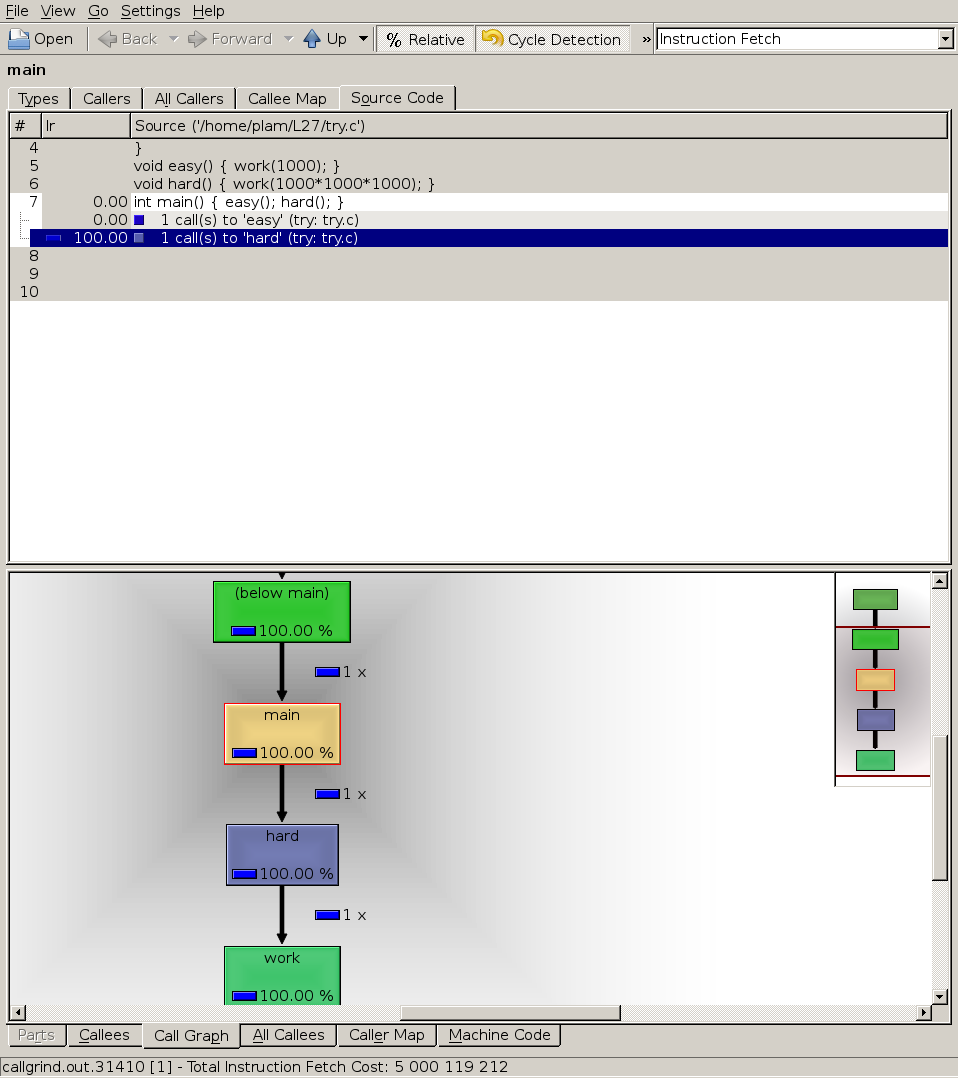
\includegraphics[width=.5\textwidth]{L27/kcachegrind}
  \end{center}
  \begin{changemargin}{2cm}
    Yes, {\tt hard} takes all the time.
  \end{changemargin}
\end{frame}
%%%%%%%%%%%%%%%%%%%%%%%%%%%%%%%%%%%%%%%%%%%%%%%%%%%%%%%%%%%%%%%%%%%%%%%%%%%%%%%%

%%%%%%%%%%%%%%%%%%%%%%%%%%%%%%%%%%%%%%%%%%%%%%%%%%%%%%%%%%%%%%%%%%%%%%%%%%%%%%%%
\begin{frame}[fragile]
  \frametitle{More Complex Example}

  \begin{center}
  \begin{minipage}{.7\textwidth}
\begin{lstlisting}
void worker1(int n) {
  volatile int i=0;
  while(i++<n);
}
void worker2(int n) {
  volatile int i=0;
  while(i++<n);
}
void manager(int n1, int n2) {
  worker1(n1);
  worker2(n2);
}
void project1() {
  manager(1000, 1000000);
}
void project2() {
  manager(1000000, 1000);
}
int main() {
  project1();
  project2();
}
\end{lstlisting}
  \end{minipage}
  \end{center}
  
\end{frame}
%%%%%%%%%%%%%%%%%%%%%%%%%%%%%%%%%%%%%%%%%%%%%%%%%%%%%%%%%%%%%%%%%%%%%%%%%%%%%%%%

%%%%%%%%%%%%%%%%%%%%%%%%%%%%%%%%%%%%%%%%%%%%%%%%%%%%%%%%%%%%%%%%%%%%%%%%%%%%%%%%
\begin{frame}
  \frametitle{Example explained in 2 lines}
  \begin{changemargin}{2cm}
    Now {\tt worker2} takes all the time in {\tt project1},\\
    and {\tt worker1} takes all the time in {\tt project2}.
  \end{changemargin}
\end{frame}
%%%%%%%%%%%%%%%%%%%%%%%%%%%%%%%%%%%%%%%%%%%%%%%%%%%%%%%%%%%%%%%%%%%%%%%%%%%%%%%%

%%%%%%%%%%%%%%%%%%%%%%%%%%%%%%%%%%%%%%%%%%%%%%%%%%%%%%%%%%%%%%%%%%%%%%%%%%%%%%%%
\begin{frame}
  \frametitle{What about KCacheGrind now?}
  \begin{center}
    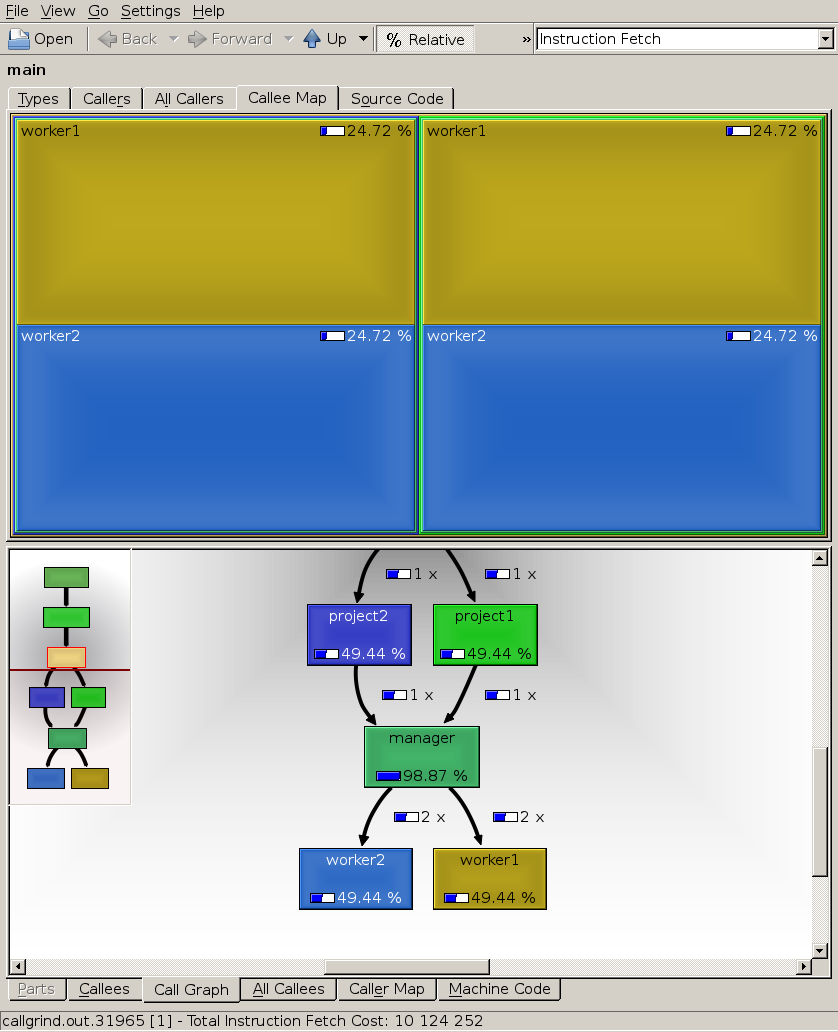
\includegraphics[width=.5\textwidth]{L27/kcachegrind2}
  \end{center}
\end{frame}
%%%%%%%%%%%%%%%%%%%%%%%%%%%%%%%%%%%%%%%%%%%%%%%%%%%%%%%%%%%%%%%%%%%%%%%%%%%%%%%%

%%%%%%%%%%%%%%%%%%%%%%%%%%%%%%%%%%%%%%%%%%%%%%%%%%%%%%%%%%%%%%%%%%%%%%%%%%%%%%%%
\begin{frame}
  \frametitle{KCacheGrind Truths}
  \begin{center}
    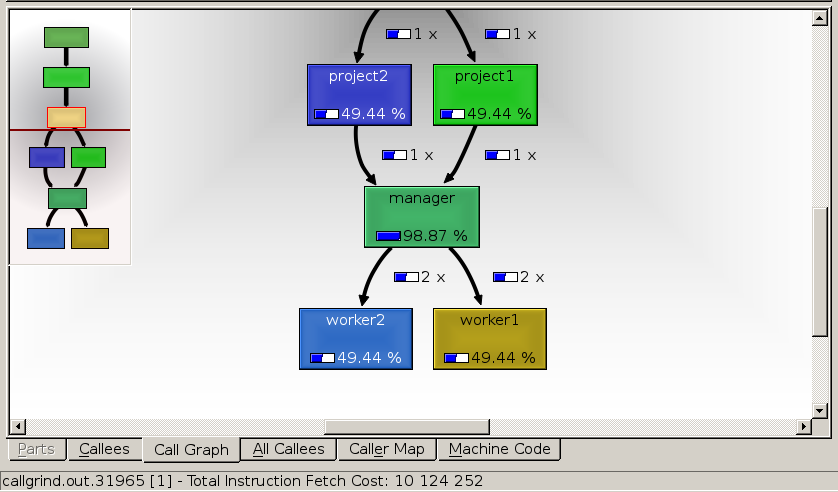
\includegraphics[width=.5\textwidth]{L27/kcachegrind2-bottom}
  \end{center}
  \begin{changemargin}{2cm}
    This is the call graph.\\
    {\tt worker1} and {\tt worker2} do each take about 50\% of time.\\
    So do {\tt project2} and {\tt project1}.\\[1em]
    (gprof would interpolate that too.)
  \end{changemargin}
\end{frame}
%%%%%%%%%%%%%%%%%%%%%%%%%%%%%%%%%%%%%%%%%%%%%%%%%%%%%%%%%%%%%%%%%%%%%%%%%%%%%%%%

%%%%%%%%%%%%%%%%%%%%%%%%%%%%%%%%%%%%%%%%%%%%%%%%%%%%%%%%%%%%%%%%%%%%%%%%%%%%%%%%
\begin{frame}
  \frametitle{KCacheGrind Lies}
  \begin{center}
    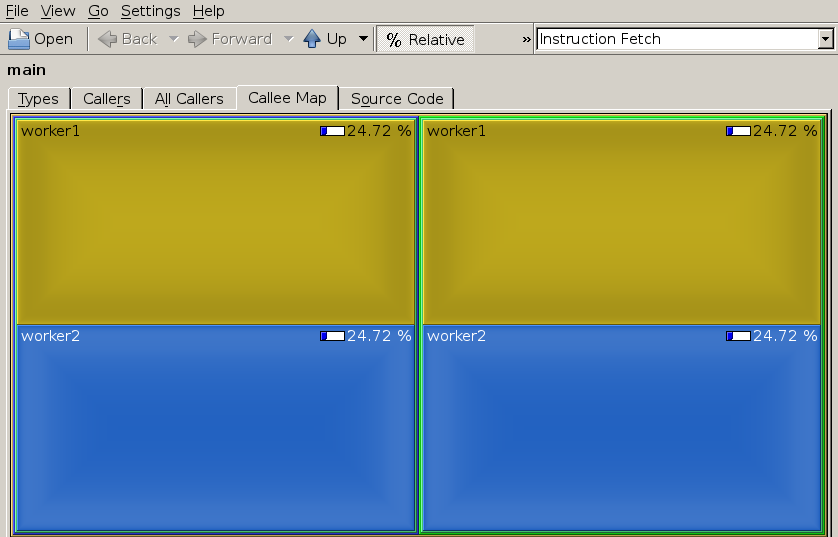
\includegraphics[width=.5\textwidth]{L27/kcachegrind2-top}
  \end{center}
  \begin{changemargin}{2cm}
    KCacheGrind is reporting:
    \begin{itemize}
    \item {\tt worker1} and {\tt worker2} doing \\
      half the work in each project.
    \end{itemize}
    That's not what the code says.
  \end{changemargin}
\end{frame}
%%%%%%%%%%%%%%%%%%%%%%%%%%%%%%%%%%%%%%%%%%%%%%%%%%%%%%%%%%%%%%%%%%%%%%%%%%%%%%%%

%%%%%%%%%%%%%%%%%%%%%%%%%%%%%%%%%%%%%%%%%%%%%%%%%%%%%%%%%%%%%%%%%%%%%%%%%%%%%%%%
\begin{frame}
  \frametitle{Why KCacheGrind Lies}

  \begin{changemargin}{2cm}
  \item gprof reports time spent in {\tt f()} and {\tt g()},\\
    and how many times {\tt f()} calls {\tt g()}.
  \item callgrind also reports \\
     time spent  in {\tt g()}
     when called from {\tt f()}, \\
     i.e. some calling-context information.\\[1em]
   \item callgrind does \emph{not} report time spent in {\tt g()} \\
     when
     called from {\tt f()} when called from {\tt h()}.\\[1em]
     We don't get the {\tt project1} to {\tt manager} to {\tt worker1} link.\\[1em]
     \item (We have Edges but need Edge-Pairs).
  \end{changemargin}
\end{frame}
%%%%%%%%%%%%%%%%%%%%%%%%%%%%%%%%%%%%%%%%%%%%%%%%%%%%%%%%%%%%%%%%%%%%%%%%%%%%%%%%

%%%%%%%%%%%%%%%%%%%%%%%%%%%%%%%%%%%%%%%%%%%%%%%%%%%%%%%%%%%%%%%%%%%%%%%%%%%%%%%%
\begin{frame}
  \frametitle{gprof/KCacheGrind summary}
  \begin{changemargin}{2cm}
    Some results are exact;\\
    some results are sampled;\\
    some results are interpolated.\\[1em]

    If you understand the tool, \\
    you understand where it can go wrong.\\[1em]

    Understand your tools!
  \end{changemargin}
\end{frame}
%%%%%%%%%%%%%%%%%%%%%%%%%%%%%%%%%%%%%%%%%%%%%%%%%%%%%%%%%%%%%%%%%%%%%%%%%%%%%%%%

\part{Lies from Metrics}

%%%%%%%%%%%%%%%%%%%%%%%%%%%%%%%%%%%%%%%%%%%%%%%%%%%%%%%%%%%%%%%%%%%%%%%%%%%%%%%%
\begin{frame}
  \partpage
\end{frame}
%%%%%%%%%%%%%%%%%%%%%%%%%%%%%%%%%%%%%%%%%%%%%%%%%%%%%%%%%%%%%%%%%%%%%%%%%%%%%%%%

%%%%%%%%%%%%%%%%%%%%%%%%%%%%%%%%%%%%%%%%%%%%%%%%%%%%%%%%%%%%%%%%%%%%%%%%%%%%%%%%
\begin{frame}
  \frametitle{Lying perf counters}
  
  \begin{changemargin}{2cm}
    While app-specific metrics can lie too,\\
    mostly we'll talk about CPU perf counters.
  \end{changemargin}

  \begin{center}
    Reference: Paul Khuong,\\
  \tiny
  \url{http://www.pvk.ca/Blog/2014/10/19/performance-optimisation-~-writing-an-essay/}

  \end{center}

\end{frame}
%%%%%%%%%%%%%%%%%%%%%%%%%%%%%%%%%%%%%%%%%%%%%%%%%%%%%%%%%%%%%%%%%%%%%%%%%%%%%%%%

%%%%%%%%%%%%%%%%%%%%%%%%%%%%%%%%%%%%%%%%%%%%%%%%%%%%%%%%%%%%%%%%%%%%%%%%%%%%%%%%
\begin{frame}
  \frametitle{mfence}

  \begin{changemargin}{1.5cm}
    We've talked about {\tt mfence}.\\
    Used in spinlocks, for instance.\\[2em]
    Profiles said: spinlocking didn't take much time.\\
    Empirically: eliminating spinlocks = better than expected!
    
  \end{changemargin}
  
\end{frame}
%%%%%%%%%%%%%%%%%%%%%%%%%%%%%%%%%%%%%%%%%%%%%%%%%%%%%%%%%%%%%%%%%%%%%%%%%%%%%%%%

%%%%%%%%%%%%%%%%%%%%%%%%%%%%%%%%%%%%%%%%%%%%%%%%%%%%%%%%%%%%%%%%%%%%%%%%%%%%%%%%
\begin{frame}
  \frametitle{Exploring the lie}

  \begin{changemargin}{2cm}
    Next step: crate microbenchmarks.\\[1em]
    Memory accesses to uncached locations,\\
    or computations,\\[1em]
    surrounded by store pairs/mfence/locks.\\[1em]
    Use perf to evaluate impact of mfence vs lock.
  \end{changemargin}

\end{frame}
%%%%%%%%%%%%%%%%%%%%%%%%%%%%%%%%%%%%%%%%%%%%%%%%%%%%%%%%%%%%%%%%%%%%%%%%%%%%%%%%

%%%%%%%%%%%%%%%%%%%%%%%%%%%%%%%%%%%%%%%%%%%%%%%%%%%%%%%%%%%%%%%%%%%%%%%%%%%%%%%%
\begin{frame}[fragile]
  \frametitle{perf for lock}

    \begin{lstlisting}
$ perf annotate -s cache_misses
[...]
    0.06 :        4006b0:       and    %rdx,%r10
    0.00 :        4006b3:       add    $0x1,%r9
    ;; random (out of last level cache) read
    0.00 :        4006b7:       mov    (%rsi,%r10,8),%rbp
   30.37 :        4006bb:       mov    %rcx,%r10
    ;; foo is cached, to simulate our internal lock
    0.12 :        4006be:       mov    %r9,0x200fbb(%rip)
    0.00 :        4006c5:       shl    $0x17,%r10
    [... Skipping arithmetic with < 1% weight in the profile]
    ;; locked increment of an in-cache "lock" byte
    1.00 :        4006e7:       lock incb 0x200d92(%rip)
   21.57 :        4006ee:       add    $0x1,%rax
    [...]
    ;; random out of cache read
    0.00 :        400704:       xor    (%rsi,%r10,8),%rbp
   21.99 :        400708:       xor    %r9,%r8
    [...]
    ;; locked in-cache decrement
    0.00 :        400729:       lock decb 0x200d50(%rip)
   18.61 :        400730:       add    $0x1,%rax
    [...]
    0.92 :        400755:       jne    4006b0 <cache_misses+0x30>
    \end{lstlisting}


\end{frame}
%%%%%%%%%%%%%%%%%%%%%%%%%%%%%%%%%%%%%%%%%%%%%%%%%%%%%%%%%%%%%%%%%%%%%%%%%%%%%%%%

%%%%%%%%%%%%%%%%%%%%%%%%%%%%%%%%%%%%%%%%%%%%%%%%%%%%%%%%%%%%%%%%%%%%%%%%%%%%%%%%
\begin{frame}
  \frametitle{lock's effects}

  \begin{changemargin}{2cm}
    Reads take 30 + 22 = 52\% of runtime\\
    Locks take 19 + 21 = 40\%.
  \end{changemargin}

\end{frame}
%%%%%%%%%%%%%%%%%%%%%%%%%%%%%%%%%%%%%%%%%%%%%%%%%%%%%%%%%%%%%%%%%%%%%%%%%%%%%%%%

%%%%%%%%%%%%%%%%%%%%%%%%%%%%%%%%%%%%%%%%%%%%%%%%%%%%%%%%%%%%%%%%%%%%%%%%%%%%%%%%
\begin{frame}[fragile]
  \frametitle{perf for mfence}

  \begin{lstlisting}
$ perf annotate -s cache_misses
[...]
    0.00 :        4006b0:       and    %rdx,%r10
    0.00 :        4006b3:       add    $0x1,%r9
    ;; random read
    0.00 :        4006b7:       mov    (%rsi,%r10,8),%rbp
   42.04 :        4006bb:       mov    %rcx,%r10
    ;; store to cached memory (lock word)
    0.00 :        4006be:       mov    %r9,0x200fbb(%rip)
    [...]
    0.20 :        4006e7:       mfence 
    5.26 :        4006ea:       add    $0x1,%rax
    [...]
    ;; random read
    0.19 :        400700:       xor    (%rsi,%r10,8),%rbp
   43.13 :        400704:       xor    %r9,%r8
    [...]
    0.00 :        400725:       mfence 
    4.96 :        400728:       add    $0x1,%rax
    0.92 :        40072c:       add    $0x1,%rax
    [...]
    0.36 :        40074d:       jne    4006b0 <cache_misses+0x30>
  \end{lstlisting}

\end{frame}
%%%%%%%%%%%%%%%%%%%%%%%%%%%%%%%%%%%%%%%%%%%%%%%%%%%%%%%%%%%%%%%%%%%%%%%%%%%%%%%%

%%%%%%%%%%%%%%%%%%%%%%%%%%%%%%%%%%%%%%%%%%%%%%%%%%%%%%%%%%%%%%%%%%%%%%%%%%%%%%%%
\begin{frame}
  \frametitle{mfence's effects}

  \begin{changemargin}{2cm}
    Looks like the reads take 85\% of runtime,\\
    while the mfence takes 15\% of runtime.
  \end{changemargin}

\end{frame}
%%%%%%%%%%%%%%%%%%%%%%%%%%%%%%%%%%%%%%%%%%%%%%%%%%%%%%%%%%%%%%%%%%%%%%%%%%%%%%%%

%%%%%%%%%%%%%%%%%%%%%%%%%%%%%%%%%%%%%%%%%%%%%%%%%%%%%%%%%%%%%%%%%%%%%%%%%%%%%%%%
\begin{frame}
  \frametitle{Bigger picture}

  \begin{changemargin}{2cm}
    Must also look at total \# of cycles.\\[1em]
    \begin{tabular}{lr}
    No atomic/fence:& 2.81e9 cycles\\
    lock inc/dec: & 3.66e9 cycles\\
    mfence: & 19.60e9 cycles
    \end{tabular}
~\\[1em]
    That 15\% number is a total lie.
  \end{changemargin}

\end{frame}
%%%%%%%%%%%%%%%%%%%%%%%%%%%%%%%%%%%%%%%%%%%%%%%%%%%%%%%%%%%%%%%%%%%%%%%%%%%%%%%%

%%%%%%%%%%%%%%%%%%%%%%%%%%%%%%%%%%%%%%%%%%%%%%%%%%%%%%%%%%%%%%%%%%%%%%%%%%%%%%%%
\begin{frame}
  \frametitle{Conclusions}

  \begin{changemargin}{2cm}
    \begin{itemize}
    \item mfence underestimated;
      \item lock overestimated.
    \end{itemize}
    ~\\
    Why? \\[1em]
    mfence = pipeline flush,\\
    costs attributed to instructions being flushed.\\
  \end{changemargin}

\end{frame}
%%%%%%%%%%%%%%%%%%%%%%%%%%%%%%%%%%%%%%%%%%%%%%%%%%%%%%%%%%%%%%%%%%%%%%%%%%%%%%%%

%%%%%%%%%%%%%%%%%%%%%%%%%%%%%%%%%%%%%%%%%%%%%%%%%%%%%%%%%%%%%%%%%%%%%%%%%%%%%%%%
\begin{frame}
  \frametitle{Summary}
  \begin{changemargin}{2cm}
    Saw a bunch of lies today:\\
    \begin{itemize}
    \item calling-context lies;
    \item perf attribution lies.
    \end{itemize}
  \end{changemargin}
\end{frame}
%%%%%%%%%%%%%%%%%%%%%%%%%%%%%%%%%%%%%%%%%%%%%%%%%%%%%%%%%%%%%%%%%%%%%%%%%%%%%%%%

\end{document}
